
\documentclass[a4paper,oneside, draft]{memoir}
\usepackage[T1]{fontenc}
\usepackage[utf8]{inputenc}
\usepackage[english]{babel}

% bedre orddeling Gør at der som minimum skal blive to tegn på linien ved
% orddeling og minimum flyttes to tegn ned på næste linie. Desværre er værdien
% anvendt af babel »12«, hvilket kan give orddelingen »h-vor«.
\renewcommand{\englishhyphenmins}{22} 

\usepackage{colortbl}  % Bruges til at farve celler, rækker mv. i tabeller
\usepackage{pdflscape} % Gør landscape-environmentet tilgængeligt
\usepackage{fixme}     % Indsæt "fixme" noter i drafts.
\usepackage{hyperref}  % Indsæter links (interne og eksterne) i PDF
\usepackage{graphicx}

\renewcommand{\ttdefault}{pcr} % Bedre typewriter font
%\usepackage[sc]{mathpazo}     % Palatino font
\renewcommand{\rmdefault}{ugm} % Garamond
%\usepackage[garamond]{mathdesign}

%\overfullrule=5pt
%\setsecnumdepth{part}
\setcounter{secnumdepth}{-1} % Sæt overskriftsnummereringsdybde. Disable = -1.

\newcommand{\EDSL}{EDSL (Embedded Domain Specific Language) \renewcommand{\EDSL}{ EDSL }}

\title{Controlling embedded devices with funktional reactive programming}

\author{Martin Dybdal (dybber@dybber.dk), \\
Jesper Reenberg (jesper.reenberg@gmail.com) \\ og
Troels Henriksen (athas@sigkill.dk)}

\date{\today}
\pagestyle{plain}



\begin{document}
\maketitle

\begin{abstract}
  Robots are conventionally programmed in low-level imperative
  languages with no concepts like events, synchronicity or any of the
  advantages found in functional programming languages (like pattern
  matching). Reactive programming languages embedded in Haskell, like
  Frob \cite{frob99} and Yampa \cite{arrowsrobotsfrp02}, has been
  suggested for robot programming, but they require a complete Haskell
  runtime system, which is to large to fit on more
  resource-constrained devices. 

  We tie these two ends together, creating a highly declarative
  language for robot programming using a staged compilation-strategy
  like the one found in Flask \cite{flask08}, that makes it possible
  to run programs on devices with few resources. In the creation we've
  used the Flask-codebase as a starting point and huge parts of the
  code is left unchanged.
\end{abstract}

\section{Disposition}
\begin{itemize}
\item Abstract

\item Preface

\item Introduction
  \begin{itemize}
  \item Brief intro to robot programming
    \begin{itemize}
     \item Sensors and Actuators
    \end{itemize}
  \item Brief Arduino introduction
  \item Brief Flask introduction
    \begin{itemize}
     \item The staged compilation strategy
    \end{itemize}
  \end{itemize}

\item Related Work
  \begin{itemize}
  \item Frob
  \item Esterel
    (http://www.softwaresafety.net/Esterel.org/esterel.html)
  \item Lustre \cite{lustre91}
  \item Flask
  \end{itemize}

\item "`Our system"'
  \begin{itemize}
  \item Staged compilation
  \item Dataflows
  \item Node representation
  \item Devices
  \item Interrupts
  \item Events
  \end{itemize}

\item Example programs

\item Conclusions

\item Bibliography

\item Appendixes
  \begin{itemize}
  \item A Flask tour
  \item Small guide to Arduino and electronics
  \end{itemize}
\end{itemize}  



\chapter{Preface}
This paper is written as a 15 ECTS Bachelor project at the Computer
Science Department (DIKU), University of Copenhagen. The authors are
Martin Dybdal, Troels Henriksen and Jesper Reenberg. The project is
supervised by Ken Friis Larsen, assistant professor at DIKU.

\fixme{maybe add thanks to Flask-guys}


\chapter{Introduction}
Production cost falling => cheaper robots => more robots to be
programmed. Fast prototyping and re-usability are important for the
industry.

...

Reactive programming and the dataflow looks like a good candidate for
programming these systems...


\chapter{Implementation}

The essence of Fladuino can be condensed to a single, conceptually
simple problem: translate a high-level functional reactive program to
a form suitable for execution on the Arduino platform.  We have chosen
to stop a step short, and merely generate C code meant for further
compilation through an Arduino-specific compiler.  We have no need of
the additional power we would gain through generating our own machine
code, and the additional amount of work required would be very large.
Flask chooses the same approach, in that it produces NesC--code for
running on sensor motes, likely for the same reasons.

Our target platform, Arduino, imposes constraints on the resulting
device-level code.  In particular, the low amount of available main
memory, and the comparatively large amount of available flash memory
for program code, suggests that we optimise for low memory usage over
low code size.  Indeed, as we shall see, we have opted to directly
express much of the control flow in the code itself, where a typical
program, with plenty of available memory, might instead choose a more
data-driven approach.

\section{Basic dataflow translation}

At their heart, both Flask and Fladuino--programs consist of an
acyclic dataflow graph.  A core part of the system involves the
translation of this high-level description of the passage of data into
the procedural target environment.  Fladuino adopts Flask's
implementation almost verbatim, the details of which will be explained
within this chapter.

As in Flask, the graph is divided into \textit{atomic subgraphs},
sections that can be executed without blocking

\subsection{Translation of a simple dataflow graph}

A set of nodes connected by a set of directed graph edges make up the
entirety of the dataflow graph.  We shall adopt the terminology of
Flask, and refer to nodes as \textit{dataflow operators} and the
directed edges as \textit{wires} in the following.  Each wire is
associated with type information regarding the values that will be
passed along it.  Some dataflow operators have no predecessor and
exist solely as entry points for data (they can be triggered by
outside events, such as device or timer interrupts), while others have
no successors and function as data sinks.  It is required that the
graph is acyclic, something that is enforced by every operator being
uniquely identified by (among other things) its predecessor(s).  A
stream operator can have multiple distinct input, but only a single
output, though this output can be split so as to send the same output
value to any number of successors.

For every operator $o$ in the dataflow graph, a set of unary
functions $o\_in_n()$ and a unary function $o\_out()$ will be
generated.  The arrival of a value $v$ at $o$ will be implemented by a
call $o\_in_n(v)$, where the exact choice depends on the wiring of the
graph.  In the typical case, even when several wires leads to a single
stream operator, there will be only a single such $o\_in_n()$
function\footnote{In fact, multiple ``in'' functions are only
  necessary for operators such as \texttt{szip}, which works by
  waiting until it has received two values $x, y$ from its two direct
  predecessors, after which it sends them along to its successors as
  the tuple $(x,y)$ --- in this case, the two functions will need
  different types and semantics, as there it is not required that $x$
  and $y$ have the same type.}.  Depending on the specific semantics
of $o$, a value $v'\equiv f(v)$ (where $f()$ represents the
computation done by $o$, the result may not even depend on $v$ at all)
may be propagated to the successors of $o$.  In this case,
$o\_in_n(v)$ will call $o\_out(v')$, the implementation of which will
feature the calls $\forall s \in S(o). s\_in(v')$, where $S(o)$ is the
set of all successors of $o$.

$o\_in()$ is generated directly by the implementation of the specific
dataflow operator, but $o\_out()$ is automatically created by Fladuino
during code generation.  The utility of this division is that the
implementation of a dataflow operator does not feature tedious
duplication of the value propagation machinery, yet as it is not
required that $o\_out()$ is called at all, each dataflow operator can
still make its own choice whether to propagate a value or not.

It is worth nothing that a value need not contain any information
apart from its existence; \texttt{()} is perfectly valid as a signal.



\bibliographystyle{plain}
\bibliography{rapport}

\appendix

\chapter{Small guide to Arduino and electronics}

\fixme{We should update the $\backslash$ texttt to uses the listings
  inline formatting instead when ever c code is listed.}

Description of Arduino from the official
website\footnote{\url{http://www.arduino.cc/} downloaded the 28. of April 2009 at 15:16}:
\begin{quotation}
  Arduino is an open-source electronics prototyping platform based on
  flexible, easy-to-use hardware and software. It's intended for
  artists, designers, hobbyists, and anyone interested in creating
  interactive objects or environments.

  Arduino can sense the environment by receiving input from a variety
  of sensors and can affect its surroundings by controlling lights,
  motors, and other actuators. The microcontroller on the board is
  programmed using the Arduino programming language (based on Wiring)
  and the Arduino development environment (based on
  Processing). Arduino projects can be stand-alone or they can
  communicate with software on running on a computer (e.g. Flash,
  Processing, MaxMSP).
\end{quotation}

\fixme{<<Image of our Duemilanove>>}

There are different kinds of Arduino boards. All are based on
different ATmega processors from Atmel. The older boards used serial
communication while the newer ones are connected to the computer
through a USB cable, but still using the same serial communication
protocol (i.e. serial through USB). The USB cable also serves as a
power supply.


We will describe the Arduino Duemilanove board we have used, in the
sections that follow, but most information will apply to
the other Arduino boards as well.

\section{Pins}
The Arduino board can connect to several external components through
diverse input and output pins. The pins are split in three physical sections on
the board \textit{power}, \textit{analog in} and
\textit{digital}. Before any IO can happen on a pin, it's mode must be
set. The mode of a pin defines if it is used to read input or
write output. The mode is set by the function \texttt{void pinMode(int
  pinnumber, int mode)} where \textit{pinnumber} is a number between
0-5 for analog and 0-13 for digital and \textit{mode} is either of the constants
\texttt{OUTPUT} or \texttt{INPUT}.

\subsection{Power pins}
% http://arduino.cc/en/Reference/Board?from=Guide.Board
\begin{itemize}
\item Reset: Resets the board when connected to ground.
\item 3V3: Constant 3,3v output
\item 5v: Constant 5v output
\item Gnd: Two ground pins
\item Vin: The voltage supplied by the external power supply.
\end{itemize}

\subsection{Digital pins}
There are 14 digital input and output pins. Six of them can also be
used to generate analog output by PWM (Pulse Width Modulation). It's
possible to read a boolean value \texttt{HIGH} and \texttt{LOW} by the
following function \texttt{bool digitalRead(int pinnumber)} where
pinnumber is a number between 0 and 13. It's possible to write a
boolean value by the following function \texttt{void digitalWrite(int
  pinnumber, int value)} where pinnumber is a number between 0 and 13
and value is either \texttt{HIGH} or \texttt{LOW}.

\subsection{Analog input}
There are 6 analog input pins. It's possible to read a voltage level
from each of them using the function \texttt{int analogRead(int
  pinnumber)} where \textit{pinnumber} is a number between 0 and 5
indicating which pin to read from. The result is given as an integer
in the range from 0 to 1023. It's possible to write a voltage level
(PWM wave, explained below) by the following function \texttt{void
  analogWrite(int pinnumber, int value)} where \textit{pinnumber} is
one of (3,5,6,9,10,11) which is located among the 14 digital pins and
\textit{value} is an integer in the range from 0 to 255. The reason
why the 6 analog output pins is located among the digital IO pins is
that the platform uses PWM to generate the desired voltage level.

\subsubsection{PWM}

A description of PWM from the Arduino website follows:
\footnote{\url{http://www.arduino.cc/en/Tutorial/PWM} downloaded the
  28. of April at 17:14}

\begin{quotation}
  Pulse Width Modulation, or PWM, is a technique for getting analog
  results with digital means. Digital control is used to create a
  square wave, a signal switched between on and off. This on-off
  pattern can simulate voltages in between full on (5 Volts) and off
  (0 Volts) by changing the portion of the time the signal spends on
  versus the time that the signal spends off. The duration of "on
  time" is called the pulse width. To get varying analog values, you
  change, or modulate, that pulse width. If you repeat this on-off
  pattern fast enough with an LED for example, the result is as if the
  signal is a steady voltage between 0 and 5v controlling the
  brightness of the LED.

  In the graphic below, the green lines represent a regular time
  period. This duration or period is the inverse of the PWM
  frequency. In other words, with Arduino's PWM frequency at about
  500Hz, the green lines would measure 2 milliseconds each. A call to
  \texttt{analogWrite()} is on a scale of 0 - 255, such that
  \texttt{analogWrite(255)} requests a 100\% duty cycle (always on),
  and \texttt{analogWrite(127)} is a 50\% duty cycle (on half the
  time) for example.

  
  \begin{figure}[h!]
    \centering
    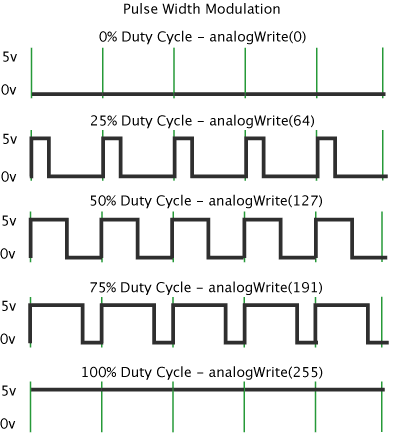
\includegraphics[scale=0.8]{images/pwm}

    \caption{How 0\%, 25\%, 50\%, 75\% and 100\% PWM is measured by a
      oscilloscope. Where Each vertical green line indicates the duty
      cycle}
    \label{fig:pwm}
  \end{figure}

  \fixme{Better figure text and figure should be non-floating. Jesper
    has a solution to this in his old Graphics report}

  Once you get this example running, grab your Arduino and shake it
  back and forth. What you are doing here is essentially mapping time
  across the space. To our eyes, the movement blurs each LED blink
  into a line. As the LED fades in and out, those little lines will
  grow and shrink in length. Now you are seeing the pulse width.
\end{quotation}


\section{Timer Interrupts}

\fixme{fix text to support new heading: timer interrupts}

The ATmega168/ATmega328 processors has three different hardware
timers. One of them (timer 0) is used by Arduino software to provide a
\texttt{millis()} function that gives us the amount of milliseconds
since the timer started and a \texttt{delay} function that actively
holds the processor occupied for a given time period. Timer 0 and 2
uses 8 bit registers and timer 1 uses a 16 bit register. This
effectively means that timer 0 and 2 can't count to more than 255
whereas timer 1 can count to 65535. The registers is incremented at
the speed of the processor, in this case 16MHz, divided by a prescale
factor which can be either of 1 (no scaleing), 8, 64, 256, 1024 for
timer 0 and 1 and either of 1, 8, 32, 64, 128, 256, 1024 for timer
2. The reason why timer 0 and 1 has 2 less prescale factors is that
they can be wired up with an external clock source and setup to
trigger on a falling or rising edge. With a prescale of 256 the
counter is incremented at a rate of $\frac{16000000\mathrm{Hz}}{256} =
62500\mathrm{Hz}$, which makes the counter overflow at a rate of
$\frac{16000000\mathrm{Hz}}{255*256} = \frac{62500\mathrm{Hz}}{255} =
245.1\mathrm{Hz}$ (pr second). This applies to all three timers where the only
2 variables are the prescale and the size of the counter register.

The three timers modes of operation is \texttt{Normal},
\texttt{CTC}(Clear Timer on Compare match), \texttt{Fast PWM},
\texttt{Phase Correct PWM} where \texttt{Normal} and \texttt{CTC} are
the ones of interrest:

\begin{description}
\item[\texttt{Normal}] mode counts from a optionally specified counter
  value (initially default set to 0) and increments until it reaches
  the maximum value 255 where it overruns, restarts from 0, the
  interrupt is triggered and incrementation of the counter
  restarts.

\item[\texttt{CTC}] mode has a predefined top value and optionally
  specified counter value (initially default set to 0). When the
  counter reaches the defined top value it is cleared to 0, the
  interrupt is triggered and incrementation of the counter
  restarts. This gives better resolution of the counter and thus more
  flexibility than the \texttt{Normal} mode.
\end{description}

The modes of operation is described in detail in the processors
datasheet, section 12.7 ``Modes of Operation''.

\subsection{PWM generation}

PWM is generated from these three timers. Pin 5 and 6 are connected to
timer 0, 9 and 10 to timer 1 and pin 3 and 11 to timer 2. This means
that the frequency of the PWM signal is controlled by the speed of
these counters which again is determined by the prescale. When an
\texttt{analogWrite(pinnumber, value)} is executed, the value is
compared against a value in a 8-bit counter (one associated to each
timer). When the counter is less than the specified value it outputs
\texttt{HIGH} on \textit{pinnumber} and \texttt{LOW} otherwise. This
generates a square wave with a duty cycle of 50\% since it is
\texttt{HIGH} on counts $0 \ldots 127$ and \texttt{LOW} on counts $128
\ldots 255$. Since Arduino uses timer 0 for the various time related
functions, the prescale on this timer can't be changed unless this
feature are not to be used. Also because of this the duty cycle of pin
5 and 6 is not exactly the same as the other 4 pins.

\fixme{Interference problems with the PWM output pins.}  

\section{External Interrupts}

Essentially all the pins on the Arduino board supports external
interrupts, though only digital pins 2 and 3 is supported directly by
the Arduino code via the function \texttt{void attachInterrupt(int
  interruptpin, void (* userfunc)(void), int mode)} where
\textit{interruptpin} is either 0 or 1, \textit{userfunc} is the user
function to call when the interrupt triggers and \textit{mode} is one
of \texttt{LOW}, \texttt{CHANGE}, \texttt{RISING} or
\texttt{FALLING}. The \textit{mode} property is special for these two
external interrupt pins, as the other pins only support the
\texttt{CHANGE} mode. The full descriptions of the modes is in the
datasheet of the processor section 10.2.1 ``EICRA - External Interrupt
Control Register A''. To set up external interrupts on the other pins
the user \textit{ckiick} has added an usable header file to the Arduino
playground\footnote{\url{http://www.arduino.cc/playground/Main/PcInt}
  taken 28. of April 2009 at 16:45} also containing an
example of how it works. This header file defines a function
\texttt{void PCattachInterrupt(int interruptpin, void (*
  userfunc)(void), int mode)} where the only difference is that the
\textit{mode} property only supports \texttt{CHANGE}.


\section{Electronics}
\fixme{Maybe a little refresher on electronics (e.g. how each
  component are drawn in a diagram, if we are going to use diagrams in
  the article). }



\end{document}
